%!TEX root = ../thesis.tex

\cleardoublepage
\chapter{Deterministic Multipath Backhaul Exposee - Masters Thesis}

\label{cha:introduction}

%%=========================================
\section{Motivation and Problem Description}
\label{sec:motivation}

One of the aims for the fifth generation of mobile networks (5G) and it's successors will be a greater diversification of the classes of service. As the use cases for these networks evolve, there is a greater need for quality of service (QoS) tailored to each use case. For example, in the Industrial Internet of Things (IIoT) the requirements on latency, jitter, and reliability may be extremely stringent. Supporting these kinds of classes of service can be a challenge for mobile network operators (MNOs) and will require novel approaches to familiar problems, such as backhaul.

As there are more heterogeneous edge deployments and more campus networks, backhaul becomes more challenging, since many sites may not have access to optical fibre, and may be forced into using other solutions such as satellite links, mmWave backhaul, or even regular ISP connetions. Providing the kind of deterministic quality of service that these sites may require can be a very difficult challenge.

Network operators may choose to utilize more than one backhaul connection at the same time, in order to increase the available bandwidth or to utilize the different qualities of the backhaul links. This bears the question whether multipathing could then be used to provide deterministic backhaul by intelligently selecting on which links to forward packets. This approach bears similarity to multihoming as well as to multi-path routing in Wireless Sensor Networks (WSNs), and can take inspiration from the existing body of research in these fields, which has demonstrated that QoS can be improved by using multiple links or paths simultaneously \cite{akella2003measurement, tao2005improving, habib2007improving, goldenberg2004optimizing, huang2008multiconstrained, akella2008performance}.


%\LTXtable{\textwidth}{tab/scenario1_sensor}

%%=========================================
\section{Goal of the Thesis}
\label{sec:goal}

\begin{figure}[h]
    \centering
        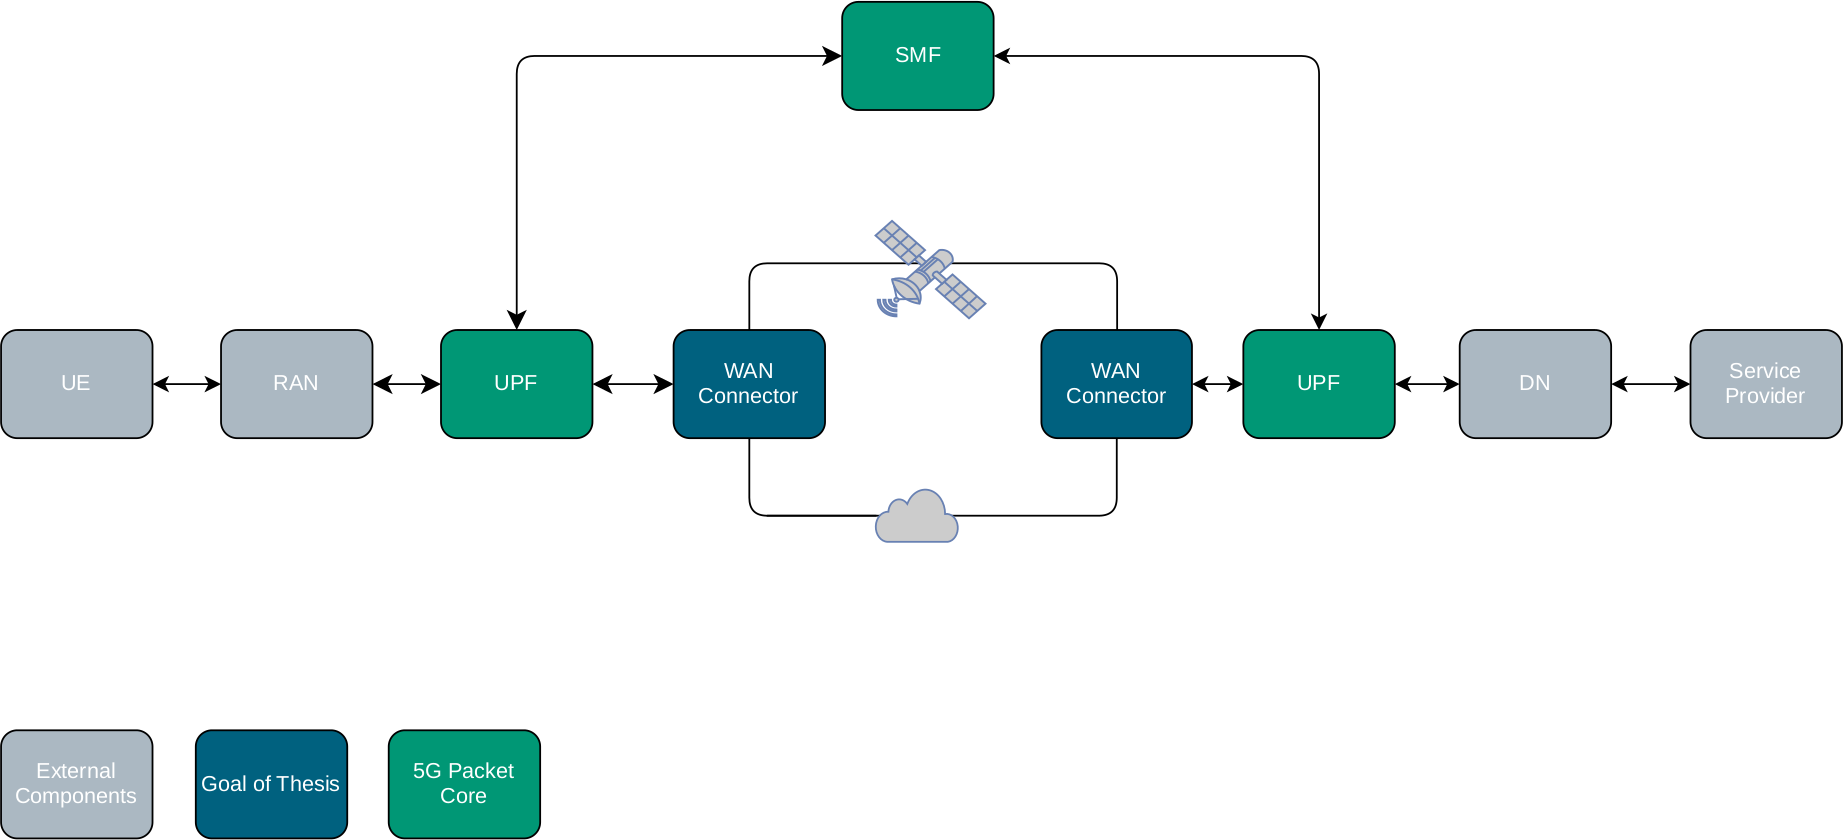
\includegraphics[width=\textwidth]{fig/telco-use-case-2.png}
        \caption{5G Deployment with 2 UPFs}
        \label{fig:telco}
\end{figure}


\begin{figure}[h]
    \centering
        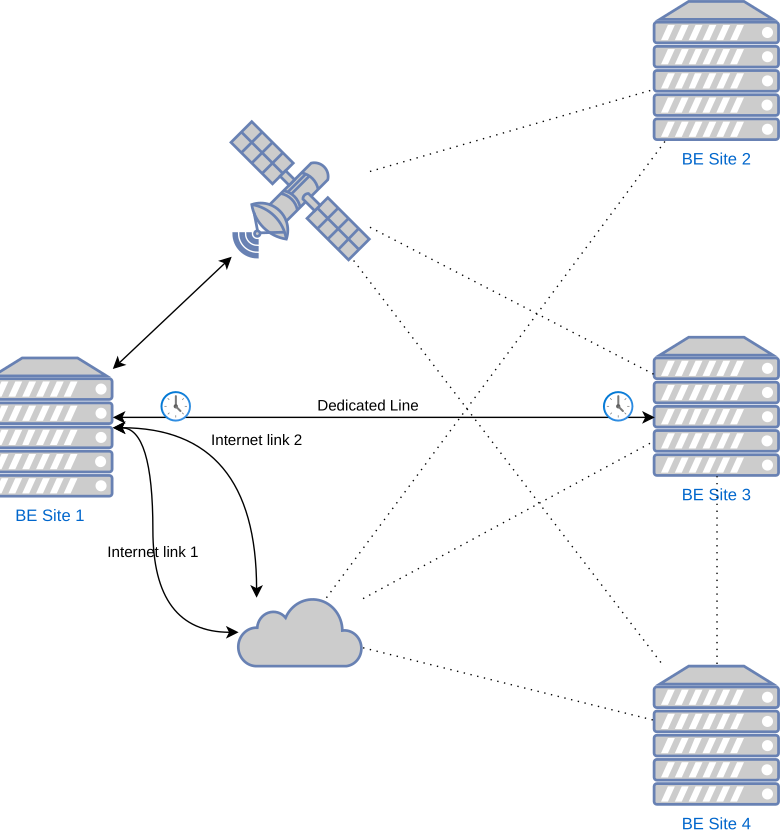
\includegraphics[width=0.9\textwidth, height=0.75\textwidth]{fig/mesh_network.png}
        \caption{Network of Backhaul Entities}
        \label{fig:mesh}
\end{figure}

The goal of this thesis is to design a backhaul entity, that can be placed at the ingress and egress point of two or more locations, and utilizes multipathing in order to provide deterministic backhaul. The performance of this approach will then be quantitatively analyzed in experiments. Looking at figures \ref{fig:telco} and \ref{fig:mesh} we can see how this is envisioned to work. Backhaul entities are deployed in 2 or more sites which have more than one egress link. Then, using the multiple outgoing links, the traffic is backhauled to the other sites, while respecting the it's QoS requirements. These entities can also be deployed in multiple sites, interconnected in a mesh network, as seen in figure \ref{fig:mesh}. This can be especially beneficial for critical applications (e.g. between industrial sites), which are in locations that don't have access to optical fibre for backhaul.

For a 5G deployment the proposed backhaul entity could be deployed between multiple User Plane Functions (UPF) and Data Networks (DNs), which also host a backhaul entity, to provide deterministic backhaul. The architecture for such a deployment is shown in figure \ref{fig:telco}.

%=======================
\section{Envisioned Approach}

The design of a backhaul entity which meets the previously listed requirements necessitates the ability to first assess the quality of the existing connections via measurements, and then choose how to forward packets along these links so as to meet the QoS requirements. These represent two distinct challenges, however the existence of useful and accurate metrics about the outgoing links is a pre-cursor for any link-selection algorithm, and thus the question of link-selection directly depends on the colleciton of accurate metrics about the outgoing links.


\subsection{Collecting Per-Link Metrics}

\subsubsection{Measurement-based Metrics}

In \cite{akella2008performance} the authors collected both passive metrics (looking at response times for outgoing packets), and active measurements (sending ICMP ping, or TCP SYN messages and measuring the response time). Using the passive measurements enabled their multihomed approach to perform well, but when using the active measurements the performance was better. Crucially, the passive measurements worked better over larger sampling periods, because it took longer to get a full overview of all the possible routes. Whereas the active sampling approach acquired it's measurements faster and was thus more effective over smaller sampling intervals.

Considering these results, it is proposed to utilize both active and passive measurements. All three metrics- packet loss, latency, and jitter- will be periodically measured in an active manner. The period over which to perform these measurements is an important design decision for the backhaul entity and it will be met later.

Beyond this, these metrics will also be monitored on a passive basis wherever possible. In order to measure either the time needed (for latency and jitter), or to ascertain that a packet has been lost, a response is required for each outgoing message. This may only be possible for TCP SYN and SYN ACK messages, and other protocols which are guaranteed to contain request-response handshakes, and thus complicates the process of passive measurement.

For classical wired links in multihomed scenarios, \cite{tao2004exploring} have observed that one link will generally dominate with regards to latency, but with brief periods where other links' performance is superior. These same authors also note that with regards to packet loss there is far less prevalence of a "dominant" link, and generally the links will perform comparably. Packet loss is also a particularly difficult metric to measure, since most links are highly reliable and when they do experience packet loss it is in bursts \cite{tao2004exploring}. Wireless connections are usually less reliable and may experience more consistent rates of packet loss at the data link layer, however it is opaque from the perspective of the higher layers, which may only perceive it through the jitter and/or latency.

 Ultimately, many of the best performing approaches for predicting packet loss, e.g. Hidden Markov Models \cite{tao2004exploring, bremler2002predicting}, are still somewhat imprecise and inaccurate. These models assume the link is in one of two states, good or bad, and each state has a different probability for packet loss, and there is a transition matrix which represents the probabilities of switching from one state to another. This thesis will also use such a model to try to predict packet loss. 

\subsubsection{Pre-configured Metrics}

To support a diversity of deployment scenarios, consideration should also be given to dedicated connections (and/or "leased lines") that may already exist at a given site. These may have hard guarantees on packet loss, latency and jitter, and this would make the measurement process for said links redundant. Therefore the backhaul entity will be designed to allow for a link to have the jitter, reliability and latency metrics pre-configured, as well as allowing their configuration to be externally updated while the entity is running.

This consideration is made because of the increasing relevance of deterministic and/or time synchronized networks (TSN) to industrial applications \cite{finn2019deterministic, zand2012wireless, tschoke2021time}, and because of the plausibility of using dedicated or leased lines to achieve similar performance \cite{tschoke2021time} in the absence of actual time synchronization. It is realistic to imagine that, in the future, 5G campus networks at remote sites may have a dedicated lines to other sites, or may be either directly connected to a TSN network or to a gateway to one. These links will usually have deterministic properties (hence the pre-configuring of metrics for the backhaul entity), and will often feature scheduled traffic \cite{finn2019deterministicarch}, which opens up interesting possibilities for backhaul.

\subsection{How to Guarantee QoS}

\subsubsection{Limiting Jitter}

The design of this approach is also an interesting challenge. One idea to improve jitter when backhauling across multiple links is to duplicate packets and forward them on multiple links, and have the backhaul entity on the other end buffer incoming packets and release them at a constant rate. This way, in the event of a packet being lost on one link, the other link is still able to receive it and the delay caused by retransmission is avoided. The downside of this approach is that it guarantees that the latency will always be as slow as the slowest link.\

\subsubsection{Low Delays}

For reducing latency it would appear likely that the simplest approach may be a greedy method (as in \cite{goldenberg2004optimizing}, in the online case) which always selects the lowest latency connection. However there is room for nuance here since the connection must not be overloaded and also because certain traffic may have very relaxed latency requirements but use up more bandwidth. This means monitoring the load on any one link will be important. Finally there are also more intelligent approaches, i.e. integer linear programming (used in \cite{huang2008multiconstrained}, and used for the offline case in \cite{goldenberg2004optimizing}) which find an optimal solution satisfying the given requirements.

The timescale over which to use a chosen link is also of interest. In \cite{habib2007improving} the time for which a link should be used is varied based on the predicted qualities of the link. These predictions are made based on past performance.

\subsubsection{Error Rates}

Reliability presents yet another challenge. However in a multihomed scenario it becomes easier to guarantee this via duplication, and/or forward error correction (FEC). For example if a packet flow requires 99\% reliability this can be guaranteed by duplicating packets across two links which are both only 90\% reliable. Alternatively, in such a situation, an FEC configured for 10\% packet loss could be used to pre-code the packets sent across one of the links, and thus increase the reliability to the required level.

Although duplication uses a lot of bandwidth, in order to support 5G's ultra-reliable low latency (URRLC) QoS requirements, which are especially relevant for IIoT applications, it may be the only option for certain traffic flows. Forward Error Correction is an excellent protection against consistently lossy links, however it may fail to be reliable when there are concentrated bursts of dropped packets, which is a more common occurrence in packet switched networks. Either way, the effectivity of FEC in a deterministic backhaul unit is an interesting question which this thesis may also explore.


\subsubsection{Proposed Solution}

The solution proposed for solving this multi-constrained QoS problem is to use integer linear programming (ILP). Although ILP is an NP-Complete Problem, we can parameterize the problem by the number of outgoing links, since this is usually small anyways and because diminishing returns set in after more than 4 links \cite{akella2003measurement}, and thus brute force the solutions.

The ILP constrained problem will be to select those links on which to forward packets while minimizing the overall number of links used, and making sure to satisfy the latency, jitter and reliability requirements of the given flow.

\begin{gather}
\text{Minimize } \sum_{i=1}^{P}x_i \\
\text{Where, } d(i) * x_i\le D \\
j(i) * x_i \le J \\
\text{and }1 - \prod_{i=1}^{P}{ ( 1- r(i) * x_i ) } \ge R  \\
\text{for } x_i \in \{0,1\}
\end{gather}

Here the variables $D$, $J$, and $R$ are the flow's delay, jitter, and reliability requirements, while the functions $d(i)$, $j(i)$, $r(i)$ are the predicted delay, jitter, and reliability of link $i$. The predicted values will usually just be the latest measurement, as recommended in \cite{akella2008performance}, however there is room here to use more advanced metrics to predict the future link quality and thus perform preemptive path switching. The total number of links is $P$. The $x_i$ variable indicates whether or not link $i$ shall be used. If a solution is found, then the flow's packets will be forwarded on each link $i$ where $x_i = 1$, and if no solution can be found which satisfies these conditions then the flow is rejected because its QoS cannot be guaranteed.

\begin{figure}[h]
    \centering
        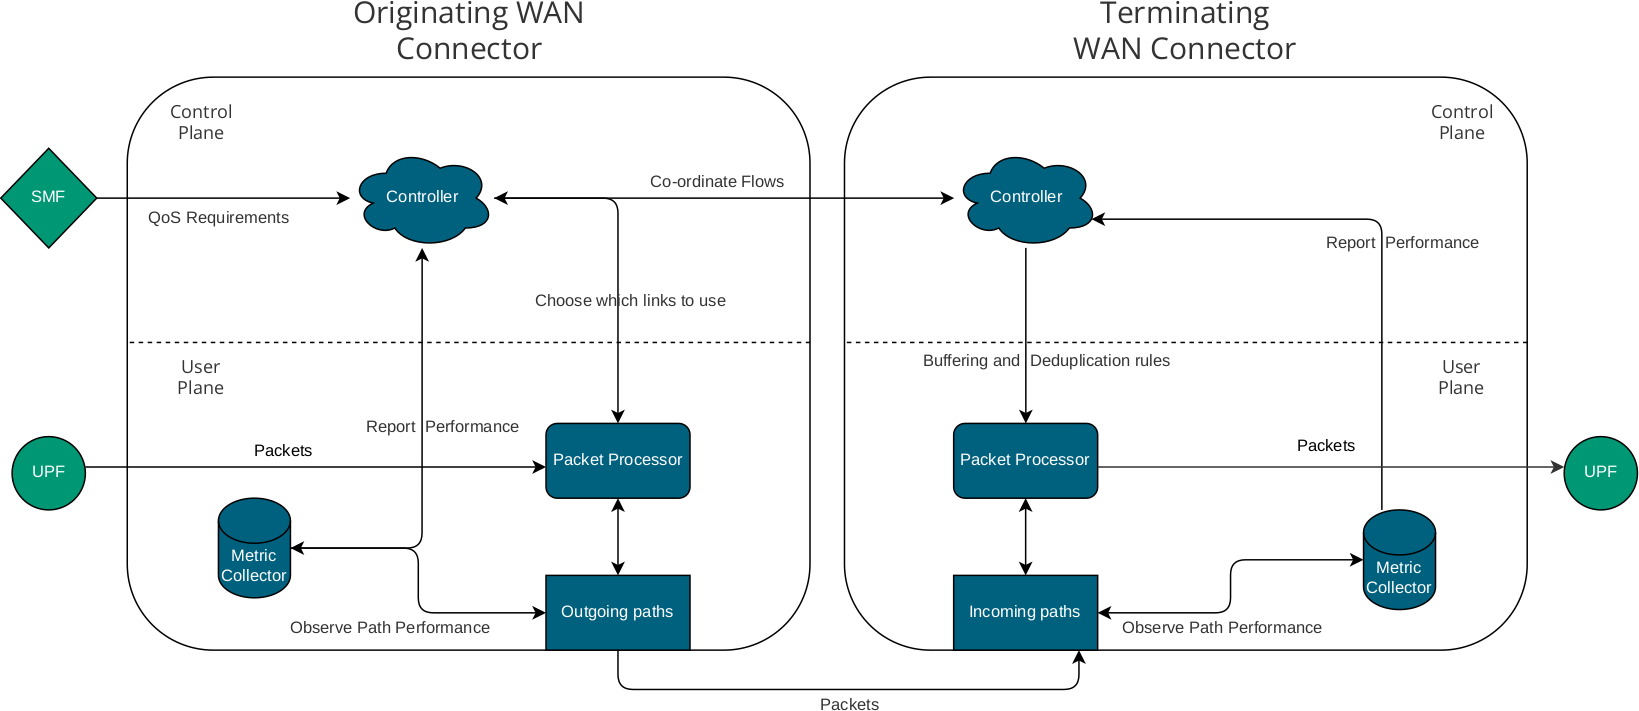
\includegraphics[width=\textwidth]{fig/be-architecture.png}
        \caption{Internal Architecture of the Backhaul Entity}
        \label{fig:arch}
\end{figure}

The proposed architecture of the backhaul entity is shown in figure \ref{fig:arch}. The backhaul entity is split into a control plane, which intelligently chooses which interfaces to forward on, and a data plane, which performs the forwarding, as well as any necessary buffering or en/decoding for forward error correction. The backhaul entity also performs different tasks depending on whether it is the origin or termination of a flow. For example, the terminating node may be receiving duplicate packets on the other paths, and it must know to drop these. Or, for example, it may need to wait and accumulate packets before releasing them at a steady rate, in order to reduce jitter (at the cost of higher latency).

Built into this architecture is a module which collects and stores data about the different links, e.g. their latency, reliability, and jitter. When polled, this module reports the performance, and may also try to predict future performance. The link selector uses this information to make its decisions.

\subsection{Potential Issues and Design Questions which are Still Open}

At present the idea would be to use the GTP protocol to tunnel data between any two backhaul entities, and then use the tunnel endpoint IDs (TEIDs) to differentiate between different traffic flows. In the control plane of the backhaul entity, one link would be chosen to be used for control and co-ordination messages between the two backhaul entities.

This approach could run into trouble if there is fragmentation. Some applications attempt to base their packet sizes on the most common MTU values for ethernet links (1500 bytes  minus 20 bytes for the IPv4 header and 2 bytes for UDP), and this causes a problem when the packet is tunneled because the overhead of another IP header on top of the tunnel header pushes the packet beyond the MTU and thus it has to be fragmented, which can degrade performance. In the proposed design of the testbed, there is a traffic generator at use, so this generator can be configured not to generate packets exceeding 1450 bytes, but this issue is of practical concern for any realistic deployments.

\subsection{Evaluating Performance}

In order to evaluate the success of the proposed approach, three scenarios will be set up and investigated. Each setup will consist of two backhaul entities, and some number of emulated links going between them. The first scenario will feature 2 WAN links, a dedicated line, and a satellite connection. The second scenario will be almost identical to the first but it won't feature the dedicated line, since it is expected that a leased line may be too obvious a choice for any of the traffic with strict QoS requirements. Finally, in order to further investigate these situations where there is an obviously superior candidate, the third scenario will just feature two links: a dedicated line and a WAN link.

\begin{figure}[h]
    \centering
        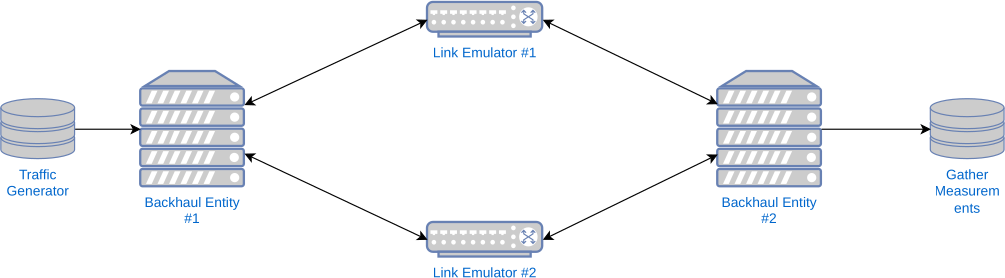
\includegraphics[width=\textwidth]{fig/testbed.png}
        \caption{Testbed Setup}
        \label{fig:testbed}
\end{figure}

In all of these scenarios the same traffic flows will be replayed. This traffic will contain various types of flows, with various QoS requirements. Before a new flow is started, the flow's requirements are sent to the backhaul entity and it is either accepted or rejected. During the traffic replay, the delay, jitter, and reliability will be measured.

These measurements will be performed once with the ILP approach proposed earlier and once with a simple round-robin approach for selecting links, and finally compared against an offline approach, where the optimal decision is computed with complete knowledge of the future. This offline approach will serve as the baseline for optimal performance, with which the other two approaches can be compared.

All of these tests can be performed on the same testbed which will be set up as show in figure \ref{fig:testbed}. The testbed architecture features a traffic generator, two backhaul entities, with a link emulator between them, and a measurement module to analyse performance. In practice the traffic generator and the test bench will be co-located on the same machine.

%%=========================================
\section{Structure of the Thesis}
\label{sec:structure}

The planned work for the thesis will be structured as follows:

\begin{enumerate}
\item{\textit{Design}: Research existing approaches and solutions, and design an approach for reliable backhaul over multiple paths/links}
\item{\textit{Implementation}: Implement said approach in a basic testbed consisting of a traffic generator, various link emulators, measurement devices, and the backhaul entities}
\item{\textit{Evaluation}: Analyse the performance of the backhaul entity according to its ability to reduce latency, improve jitter, and provide any other QoS requirements. Then compare it's performance with that of the individual links, as well as that of the other approaches.}

\end{enumerate}

The structure of the document will be a simple five chapter format: 1) Introduction, 2) Background and Related Work, 3) Approach, 4) Evaluation, 5) Conclusion. The approach chapter will discuss the proposed solution, and the evaluation chapter will encompass the design of the testbed and an analysis of the results.

\subsection{Timescale}

A thesis should take 6 months, or roughly 26 weeks. At present it is proposed to divide those 26 weeks into 4 equal sized chunks. The first 3 chunks will correspond to the 3 items mentioned previously in this section, the final "chunk" will be to finish writing up the report, however it is planned to do some writing during the other 3 chunks as well. In the first period - the \textit{Design} period, chapters 1 and 2 will also be worked on. After the \textit{Implementation} period is finished, chapter 3 can be written. Chapters 4 and 5 can then be written after the \textit{Evaluation} period finishes. That leaves the final chunk of time, which can be used to revise the document, as well as acting as a buffer in case other parts of the thesis take longer.


\begin{figure}
\begin{ganttchart}[expand chart=\textwidth, vgrid, hgrid]{1}{26}
  \gantttitle{Week}{26} \\
  \gantttitlelist{1,...,26}{1} \\
%  \ganttgroup{Group 1}{1}{7} \\
  \ganttbar{Literature Review}{1}{2}  \ganttbar[bar/.append style={fill=lightgray}]{}{3}{4} \\
  \ganttbar{Setup Testbed}{2}{4} \\
  \ganttbar{Implement Approach}{4}{8}] \ganttbar[bar/.append style={fill=lightgray}]{}{9}{10}  \\
  %ganttbar[bar/.append style={fill=lightgray}]{}{14}{14} \\
  \ganttbar{Metric Collection}{5}{7} \\
  \ganttbar{Link Switching Algorithm}{6}{8}\\
  \ganttbar{Adjust and Improve}{7}{9} \\
  \ganttbar{Measurements}{10}{16}  \ganttbar[bar/.append style={fill=lightgray}]{}{16}{18} \\
  \ganttbar{Round Robin}{12}{14} \\
  \ganttbar{God Routing}{14}{16}  \\
  \ganttbar{Evaluation}{18}{20}  \ganttbar[bar/.append style={fill=lightgray}]{}{21}{22} \\
  \ganttbar{Finish Writing Thesis}{21}{23}  \ganttbar[bar/.append style={fill=lightgray}]{}{24}{26} \\
  % \ganttlinkedbar{Task 2}{3}{7} \ganttnewline
 % \ganttmilestone{Milestone}{7} \ganttnewline
  \ganttlink{elem2}{elem3}
  \ganttlink{elem4}{elem8}
  \ganttlink{elem5}{elem8}  
  \ganttlink{elem6}{elem8}
  \ganttlink{elem7}{elem8}

 \ganttlink{elem9}{elem12}
 \ganttlink{elem10}{elem12}
 \ganttlink{elem11}{elem12}

\ganttlink{elem12}{elem14}

\end{ganttchart}
\caption{Gantt Chart: 15.06.23 - 15.12.23}
\end{figure}

The first phase of the experimental work will consist of setting up the testbed. This means installing the measurement modules as well as the link emulators. The next phase will require the implementation of the backhaul entity, as designed. The backhaul entity will require a module for collecting per-metric links, as well as the implementation of an algorithm to select the best link or links for a given flow. In the course of designing and preparing the backhaul entity there may be room for adjusting the initial plan based on what we experience during development. Next, the entity must be tested. During this phase traffic replays will be played over the testbed and evaluated. Thereafter the round robin approach and the "god routing" approach will also be evaluated. These two approaches will serve for comparison with the performance of the backhaul entity. Finally, this data must be analyzed, and the thesis can reach its conclusions, with 1 or 2 weeks buffer room for final revisions.


%%% include all citations

% start zotero

%\nocite{kundel_user_2022}
%\nocite{goldenberg_optimizing_nodate}
%\nocite{lange_performance_2015}
%\nocite{tarique_survey_2009}
%\nocite{tschoke_time-sensitive_2021}
%\nocite{ganichev_yamr_2010}
%\nocite{habib_improving_2007}
%\nocite{tao2005improving}
%\nocite{fanglu_guo_experiences_2004}
%\nocite{akella_measurement-based_nodate}
%\nocite{noauthor_zotero_nodate}

% end zotero...


% google scholar

%\nocite{tsai2006review}
%\nocite{tao2005improving}
%\nocite{kundel2022user}
%\nocite{goldenberg2004optimizing}
%\nocite{lange2015performance}
%\nocite{tarique2009survey}
%\nocite{tschoke2021time}
%\nocite{ganichev2010yamr}
%\nocite{habib2007improving}
%\nocite{guo2004experiences}
%\nocite{akella2003measurement}
%\nocite{ergencc2021reliability}
%\nocite{tao2004application}
%\nocite{alwan2010multi}
%\nocite{prados2021asynchronous}
%\nocite{zhang2016fundamentals}
%\nocite{chen2020collaborative}
%\nocite{akella2008performance}
%\nocite{andreoli2017mobile}
%\nocite{huang2008multiconstrained}
%\nocite{capela2014multihoming}
%\nocite{sheyibani2012reliable}
%\nocite{nguyen2003path}
%\nocite{tao2004exploring}
%\nocite{bremler2002predicting}
%\nocite{zand2012wireless}
%\nocite{li2016multipath}
%\nocite{finn2019deterministic}

